\documentclass[journal]{IEEEtran}
\usepackage[hidelinks]{hyperref}
\usepackage{booktabs}
\usepackage{graphicx}
\usepackage{enumitem}
\usepackage{microtype}
\usepackage{float}
\setlength{\emergencystretch}{1em}

\title{Tokens-to-Trace: What an Agent Must Read\\Before It Can Change Your Code}
\author{Vasili Gavrilov}

\begin{document}

\maketitle

\begin{abstract}
Before an AI coding agent can change code safely it must read everything
that decides what the code does. We count that reading as
tokens-to-trace: for one entry point, the tokens of the smallest set of
source regions that determine its behavior, classified by where each
region lives: in the project, in library source outside it, or in no
file at all, only in the conventions of the version in use. Measured on
three language pairs, the plain member of each pair keeps a whole path
in a few thousand tokens inside the project; the layered member spends
124 to 283 thousand tokens outside it, or keeps part of the deciding
text where no repository holds it. In 390 controlled agent runs the
layered side cost more turns wherever a task crossed files or
conventions, and its only wrong answers came from a convention no
source file states.
\end{abstract}

\section*{The reader changed}

A class hides a representation and an interface hides an implementation.
A framework hides something larger: control flow. Each is a remedy for a
limit of human working memory. An agent is not under that limit and is
under others: the context it carries and the relationships it must
resolve before acting. A hidden implementation is a relationship to
resolve, which abstraction adds rather than removes.

The machine cost of abstraction was priced decades ago by compiler work
and the zero-overhead principle, and nothing here rests on it. The
reader's cost was never priced, and the reader has changed. Studies of
agent trajectories already show where the money goes: agents spend most
of their tokens reading, and the language with the longest programs is
not the one that costs the most \cite{tokenmax,spend}. Those are counts
of consumption, properties of a model, a harness and a date. This
article contributes the static count: a property of the code alone,
computable before anything is built or any agent runs. The measure is
the contribution; the systems measured below are demonstrations of how
to apply it, and the verdicts are theirs, not the measure's.

\section*{The measure}

Tokens-to-trace of an entry point is the token count of the minimal set
of source regions that fully determines its behavior, wire to storage
and back: routing, authentication, authorization, handler logic, query,
schema, serialization, error mapping. A region is in the set iff
removing it leaves some behavior undetermined. A platform floor (JDK,
libc, the browser engine, the database) is excluded identically
everywhere; anything the application configures, or that varies by
library version, is included. Each region is classified by residence:

\begin{enumerate}[nosep]
\item \textbf{repository}: read directly from the project's own source;
\item \textbf{library source}: text outside the repository that decides
behavior before the program runs;
\item \textbf{convention}: fixed by defaults of the exact version in
use, recoverable from its documentation or a runtime observation, not
from any source file.
\end{enumerate}

Tokens are o200k, counted with tiktoken \cite{tiktoken}: a public,
model-neutral count near what a commercial agent is billed. The measure
is a count: anyone can recompute it from the region manifests published
with the full study \cite{full}, so two systems compare by number, and a
disagreement is about a manifest row, not an interpretation. Where the
floor sits is a declared judgment, and moving it moves the numbers by a
stated factor: 2.5 for the C system below, 2.4 for the framework's
category 2. In the agent's own terms the closure is the needed context:
what must be in front of it before it can decide that a change is safe.

\section*{Six closures, three pairs}

One read path per system, each doing the same kind of work: an
authenticated or filtered list over a local store (Figure~\ref{fig:closures}).

\begin{figure}[!t]
\centering
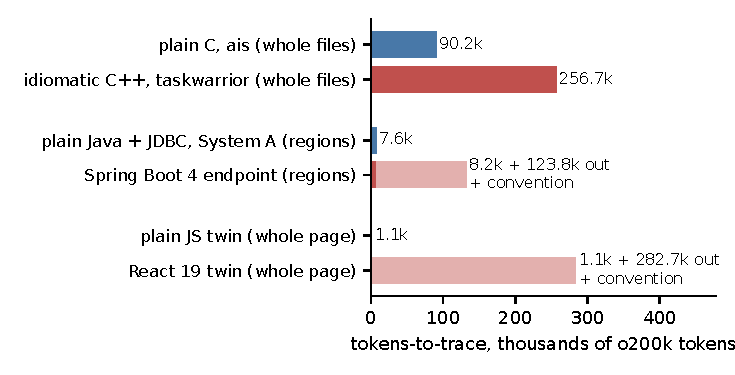
\includegraphics[width=\columnwidth]{fig_closures.pdf}
\caption{Tokens-to-trace of one read path per system, each pair at the
same counting granularity. Dark bars are text in the project's own
repository; light bars are framework source outside it; ``conv.'' marks
behavior fixed by version convention, in no file at all.}
\label{fig:closures}
\end{figure}

\textbf{C against C++.} The plain C system is ais, an associative index
of 10,597 code lines written to an explicit style guide \cite{ais}; its
recall path, argv to the bytes on disk, closes in 16 files. The C++
system is taskwarrior 2.6.2, a widely used task manager and the last
all-C++ release of its line \cite{taskwarrior}; its \texttt{task list}
closes in 99 files. Whole files on both sides: 90,151 tokens against
256,664, a factor of 2.8 in tokens and 6 in files. At region
granularity the C path is 14,444 tokens: 7\% of one 200k context
window. To bound how much of that is the author rather than the style,
the same rule applied to a library nobody here wrote, Monocypher's AEAD
encrypt path \cite{monocypher}, closes at 7,560 tokens: at the
algorithmic extreme the plain style's closure is the same few thousand
tokens whoever writes it.

\textbf{Plain Java against Spring.} System~A is a commercial web
application in production, 39,677 code lines, plain Java with JDBC,
reported anonymously. Its endpoint (token authentication, role gate,
per-object ACL, a 4-table JOIN, streamed JSON, central error mapping)
closes in 813 lines across 17 files, 7,566 tokens: 3.8\% of a window,
with categories 2 and 3 at zero, because every callee is named
literally at its call site. The framework subject is a well-regarded
Spring Boot 4 implementation of the RealWorld specification
\cite{realworld}. Its comparable endpoint needs 8,175 tokens in the
repository, 8\% more than System~A's whole closure, plus 123,794 tokens
of framework classes on the dispatch path, measured from the published
sources jars (51,342 under the most generous floor). Beneath that,
uncounted, hibernate-core alone is 6.7M tokens of source. And part of
what Spring does is written in no file at all: the derived-query
grammar that turns \texttt{findAllByAuthorProfileUserName} into a join
tree, parameter binding, filter-chain order, fetch and flush defaults.
That is category 3, and no counting granularity reaches it: a
convention that is in no repository cannot be read at any granularity.

\textbf{Plain JS against React.} Behavior-matched twins of the list
screen every application has (fetch, filter, sort, select, delete),
equal on the graded projection of the rendered DOM. The pages
themselves are the same size, 1,092 tokens against 1,145: writing
concedes nothing to JSX. Behind the React page sit 282,717 tokens of
the runtime's own source over 29 modules (the whole runtime is
641,367), 2.3 times the Spring closure.

The implicit context differs the same way. K\&R is 272 pages and
Stroustrup is 1,368 \cite{knr,stroustrup}, and a framework's reference
has no fixed size at all: what it says and how much of it there is
depend on the version, and the training corpus superposes the versions.
Window growth absorbs the C++ row's volume; it does not remove a
coherence problem.

\section*{390 runs: what the agent actually pays}

A count of text is not yet a cost. Four experiments put agents on the
measured pairs: 390 runs total, one model (claude-sonnet-5, headless),
tasks that name behavior and never a file or a function, graded by
hidden tests the agent never saw. Table~\ref{tab:stats} is the summary;
the raw run records ship with the study \cite{full}.

\begin{table}[!t]
\centering
\footnotesize\setlength{\tabcolsep}{3pt}
\begin{tabular}{@{}lrrrrr@{}}
\toprule
Experiment & Runs & Pass & Plain & Layered & $p$ \\
\midrule
C/C++ constructs, turns & 280 & 278/280 & 7.87 & 9.41 & 0.031$^{a}$ \\
Java endpoint, turns & 40 & 38/40 & 7.15 & 8.40 & 0.023$^{b}$ \\
Java endpoint, wall s & & & 24.9 & 30.2 & 0.022$^{b}$ \\
Web twins, turns & 40 & 40/40 & 6.95 & 6.85 & 0.91 \\
Web version traps & 30 & 30/30 & \multicolumn{2}{c}{0 wrong choices} & \\
\;\;its boundary task, turns & 15 & 15/15 & 6.0 & 12--13 & $^{c}$ \\
\bottomrule
\end{tabular}
\caption{The run experiments. $^{a}$C++ dearer in six of six independent
constructs, sign test. $^{b}$Permutation within task, one-sided,
100{,}000 resamples. $^{c}$Five runs per cell; cumulative context 323
and 353 thousand tokens against plain's 181, \$0.14 a run against
\$0.09. Both failures in the set are the Spring side's silent binding
miss.}
\label{tab:stats}
\end{table}

\textbf{The constructs, priced one at a time.} Six C/C++ pairs isolate
one construct each (a virtual registry, a template, operator overloads,
RAII, inheritance, a mix), same behavior, same tasks, hidden tests, 40
runs per pair. Correctness does not separate: 278 of 280 passed. Turns
do (Figure~\ref{fig:pairs}): the C++ side cost more in all seven pairs,
with three effects above the measured rerun noise: the registry spread
over eight files ($+3.50$ turns, $p = 0.003$), the mix ($+2.80$,
$p < 0.001$), the template ($+1.70$, $p = 0.004$). The control pair is
the point: the same registry classes in a single file cost $+0.50$,
indistinguishable from zero, so the agent pays for the walk across
files, not for the virtual dispatch. And held to identical behavior the
C++ text is only 1.17 times the C: the 2.8 between the whole tools is
scope and file scatter, not syntax. The experiment ran twice; on
unchanged pairs the small deltas moved (RAII $+0.50$ then $+1.05$), so
we trust the sign, the three large effects, and nothing finer.

\begin{figure}[!t]
\centering
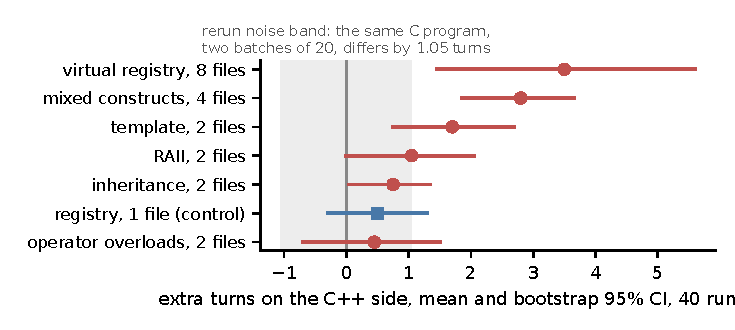
\includegraphics[width=\columnwidth]{fig_pairs.pdf}
\caption{The C/C++ pairs: extra turns on the C++ side per construct,
mean and bootstrap 95\% CI (20{,}000 resamples). The square is the
control: the eight-file registry's classes moved into one file. Effect
sizes (Cliff's $\delta$) run 0.23 to 0.80, largest for the mix and the
scattered registry.}
\label{fig:pairs}
\end{figure}

\textbf{The endpoint, two stacks.} One endpoint, an item list and item
create behind bearer-token authentication over SQL, built twice with
the same routes, schema, and observable behavior, equivalence verified
at the HTTP boundary before any run. The plain side is one file, JDK
\texttt{HttpServer} and JDBC, 108 lines; the framework side is seven
classes of current Spring idiom. Four maintenance tasks, five
repetitions each (Figure~\ref{fig:runs}). The framework side cost 1.25
turns and 5.3 seconds more per run, and gave the only wrong answers of
all 390: twice, on the filter task, the agent wrote
\texttt{@RequestParam(required = false) Integer minLen} with correct
JPQL behind it. Spring binds a query parameter by the Java parameter
name; the URL says \texttt{min\_len}; the parameter stayed null and the
endpoint returned the unfiltered list with status 200. Nothing in the
compiler, the runtime or the response flagged it. The deciding rule is
a category-3 convention, and this is what its failure looks like:
silent wrong rows. The plain side parses its query string in visible
code, so the same mistake had no place to hide, five of five. The
direction is not uniform, and the exception is instructive: on the
401-contract task Spring was cheaper, 4.2 turns against 6.0, because
its filter puts the whole authentication contract in one small class.
Where the framework localizes a change it wins the turn count; where
the behavior crosses its conventions it loses turns or correctness.

\begin{figure}[!t]
\centering
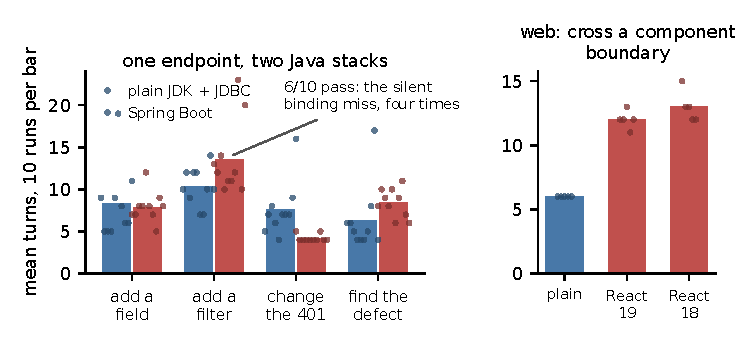
\includegraphics[width=\columnwidth]{fig_runs.pdf}
\caption{Left: the Java endpoint, mean turns per task, dots are
individual runs. Right: the web pair's boundary task, focusing a child
component's input from the parent, against React 19 and React 18.}
\label{fig:runs}
\end{figure}

\textbf{The web pair.} On four local maintenance tasks the twins did
not separate, and React won the add-a-field task, 5.6 turns against
7.6: the component boundary puts that change in one small file. Two
tasks whose correct idiom changed between React 18 and 19 produced
zero version-wrong choices in 30 runs: this model's habitual idioms
are the version-portable ones, and another model's habits need not be.
What separated is the boundary: focusing a child component's input
from the parent cost twice the turns of the unfactored plain page,
every run passing. The web pair repeats the C/C++ result, not the Java
one: nothing broke, and the agent pays for the walk across the
boundary.

\section*{The subjects are demonstrations, not samples}

One rater derived the closures, he is the author of the plain systems,
and he chose the endpoints and where the floors sit. In a sampling
study that is a flaw. This is not a sampling study, and the choices are
the method: each plain subject demonstrates how cheap a path becomes
when it is built for the new reader, the way a proof of existence picks
its witness. The demonstration is open in both directions. Write your
path plainer than these and the point strengthens; nobody claims these
witnesses are minimal. And you can always find less efficient
implementations of either style: a heavier Spring than the measured
RealWorld, a more scattered C++ than taskwarrior, and equally a C
codebase whose closure measures like taskwarrior's, since nginx-style
ops-struct vtables would resolve no more cheaply than a registry. The
style is not the language; the closure is the property, and the
language only sets how hard the low closure is to reach.

That inversion is the recommendation. Do not argue about taste: measure
the closure of one representative path in the stack you are choosing,
at a declared floor, and compare numbers. The measure costs an
afternoon with a tokenizer, and it settles which side of
Figure~\ref{fig:closures} your candidate is on before a line of the
system exists.

The low closure is also reachable on demand. An agent's default is its
training-set average, the industry idiom; one line in the prompt,
``plain C'', ``plain Java with JDBC, streaming'', ``plain vanilla
JavaScript'', steers it off that mean, and the closures above are the
result of that one-line bias. Several of the plain C projects in the
study were rewritten by an AI coder under exactly that direction
\cite{full}. The remaining human work is the objective (requirements
precise enough to implement) and the guards (what the tests must
assert); the working practices this compresses are published as recipes
\cite{recipes}.

\section*{By coincidence, it is C}

The recommendation is not a return to C, and it is not nostalgia. It
is: write in a smaller subset of whatever stack you hold, with fewer
indirections, still portable. Inside Java that subset is JDBC, visible
SQL and streamed rows, and System~A shows it runs a commercial product.
Inside the browser it is the DOM the engine already gives you, and the
twin shows it costs the same tokens to write. Inside C++ it is the part
that compiles as C. Take the subtraction to its end, a language whose
semantics have not moved in forty years, so that everything ever
written about it describes the same language and the training corpus is
one coherent body, and the language you are holding is, by coincidence,
C. The old languages were
expensive for unaided humans, and the expense was exactly the
bookkeeping agents now do.

What of abstraction's other jobs? Reuse of hard, stable code survives
fully: that is the platform floor, and the measured plain systems keep
it (the database, the cipher, the browser engine). Contracts between
teams partially survive as module seams. Compression for small working
memory loses its purpose where the whole deciding text fits beside the
work, and reliable mechanical edits, the reason for DRY, showed no
failure in a dedicated 25-run experiment at up to 30 exact-copy sites,
though the near-miss cross-file form remains untested \cite{full}.

\section*{Limits}

The numbers bound mechanisms, not laws. One rater derived the closures;
a blind second rater re-deriving two of them agreed on 97 of 103 C++
files but found 373k tokens of Spring category 2 where the printed
trace counts 124k, so the framework number is confirmed as an
undercount, and its printed form is the conservative trace. One model
ran, on one date; agent cost is a property of the model and the
representation together. The cells are five runs; every run sat far
below the context window, so what a closure that outgrows the window
costs is untested, and the volume experiment that decides it,
cross-module tasks on taskwarrior against a plain twin, is named in the
study as open. The measure prices reading and nothing else: not
security, not what a type system removes, not the certification regime
that verifies every duplicated site separately. Prior cross-language
work compares pass rates or run-time spend \cite{multiple,swebench};
tokens-to-trace is the pre-run complement, and both counts are needed,
because an agent answering from its weights makes missing context look
free.

\section*{What to do Monday}

\begin{itemize}[nosep]
\item Before choosing a stack, measure tokens-to-trace of one
representative path in each candidate, at a declared floor, and ask
where the deciding text lives. A path whose behavior rests on
convention will fail the way the filter task failed: silently.
\item When writing with an agent, state the bias in the prompt: the
plain subset of your stack, named in one line. The agent's default is
the industry average; the low closure is one sentence away.
\item Keep abstraction where a platform floor earns it, and spend the
human effort on the requirements and the tests.
\item If your path measures cheaper than the witnesses here, publish
the number. The measure is recomputable, and the comparison is the
point.
\end{itemize}

\begin{thebibliography}{9}
\bibitem{knr} B.~Kernighan, D.~Ritchie. \emph{The C Programming
Language}, 2nd ed. Prentice Hall, 1988.
\bibitem{stroustrup} B.~Stroustrup. \emph{The C++ Programming
Language}, 4th ed. Addison-Wesley, 2013.
\bibitem{taskwarrior} taskwarrior 2.6.2.
\url{https://github.com/GothenburgBitFactory/taskwarrior}.
\bibitem{realworld} \texttt{realworld-springboot-java} v2.1.1.
\url{https://github.com/raeperd/realworld-springboot-java}.
\bibitem{monocypher} L.~Vaillant. Monocypher 4.0.3.
\url{https://monocypher.org}.
\bibitem{ais} \texttt{ais}, an associative index in C99, with its style
guide under \texttt{doc/dev}. \url{https://github.com/Anode1/ais}.
\bibitem{tiktoken} tiktoken, OpenAI's tokenizer library;
\texttt{o200k\_base}. \url{https://github.com/openai/tiktoken}.
\bibitem{tokenmax} \emph{The Best Programming Language for
Tokenmaxxing: An Investigation of Coding Agent Behavior Across
Programming Languages}. arXiv:2607.22807, 2026.
\bibitem{spend} \emph{How Do AI Agents Spend Your Money? Analyzing and
Predicting Token Consumption in Agentic Coding Tasks}.
arXiv:2604.22750, 2026.
\bibitem{multiple} F.~Cassano et al. \emph{MultiPL-E: A Scalable and
Polyglot Approach to Benchmarking Neural Code Generation}. IEEE TSE,
2023.
\bibitem{swebench} C.~Jimenez et al. \emph{SWE-bench: Can Language
Models Resolve Real-World GitHub Issues?} ICLR, 2024.
\bibitem{full} V.~Gavrilov. \emph{When Abstraction Becomes Indirection:
Tokens-to-trace, Measured on Six Stacks}. Zenodo, 2026.
\url{https://doi.org/10.5281/zenodo.22113993}. Manifests, pair
programs, graders and raw run records.
\bibitem{recipes} \texttt{agent-recipes}: working practices for coding
with AI agents. \url{https://github.com/Anode1/agent-recipes}.
\end{thebibliography}

\end{document}
